% Provenance (never printed): see sources/outline_sources.md (Year 2: sedimentary basins;
% subsidence curves and backstripping; the stretching model). Stretching model after McKenzie
% (1978) as restated by Sheplev and Reverdatto (1998) and coded in pyBacktrack (EarthByte);
% backstripping after pyBacktrack's well module; North Sea after Sclater and Christie (1980);
% Michigan after Sloss (1982) and Crowe et al. (2009); the US Atlantic margin after Schlee et
% al. (1976), Poag (1979) and Lang et al. (2024); the Molasse after the chapter 13 rows.
% Curves and the invented well from figdata/bachelor-2/basins.py; exercise and problem values
% in the Book 4 scratch calculator calc/ch16.py.
\chapter{Sedimentaire bekkens vergeleken}\label{ch:b2:basins-compared}

Voor de kust van het oosten van de Verenigde Staten, onder het continentaal plat, bevat de Baltimore
Canyon Trough minstens \qty{14}{km} sedimentgesteente. Een boring in zo'n
stapel leest zijn geschiedenis achterstevoren: elke eenheid die ze doorkruist, was ooit de zeebodem, op een diepte die
fossielen en sedimenten vastleggen, en is sindsdien begraven en samengedrukt. De diepte van elk
gedateerd vlak is een punt op een dalingscurve. Toch werd het grootste deel van de daling veroorzaakt door het
gewicht van het sediment zelf. Om te weten wat het bekken maakte, moet dat gewicht eraf worden gehaald,
laag na laag. Dit hoofdstuk toont hoe, en wat het resultaat over de lithosfeer zegt.
% ledger: poag79:bct, schlee76:atlantic

\begin{recall}
\textbf{Uit Boek~3}: sedimentair bekken, subsidentie en tektonische subsidentie,
accommodatie, eustasie; compactie, decompactie en de wet van Athy, de vaste dikte van een
laag; de sedimentlast, die de subsidentie versterkt met $(\rho_m - \rho_w)/(\rho_m - \rho_s)$;
Airy-isostasie; de lithosfeer en zijn geotherm; continentale riften en passieve randen.
\textbf{Uit de natuurkundeboeken}: de warmtevergelijking en haar oplossingen van Fourier.
\textbf{Uit \cref{ch:b2:alpine-orogen}}: het \omterm{def:b2:alpine-orogen:foreland}{voorlandbekken}, \omterm{def:b2:alpine-orogen:foreland}{flysch} en \omterm{def:b2:alpine-orogen:foreland}{molasse}.
\end{recall}

\begin{omfigure}
\centering
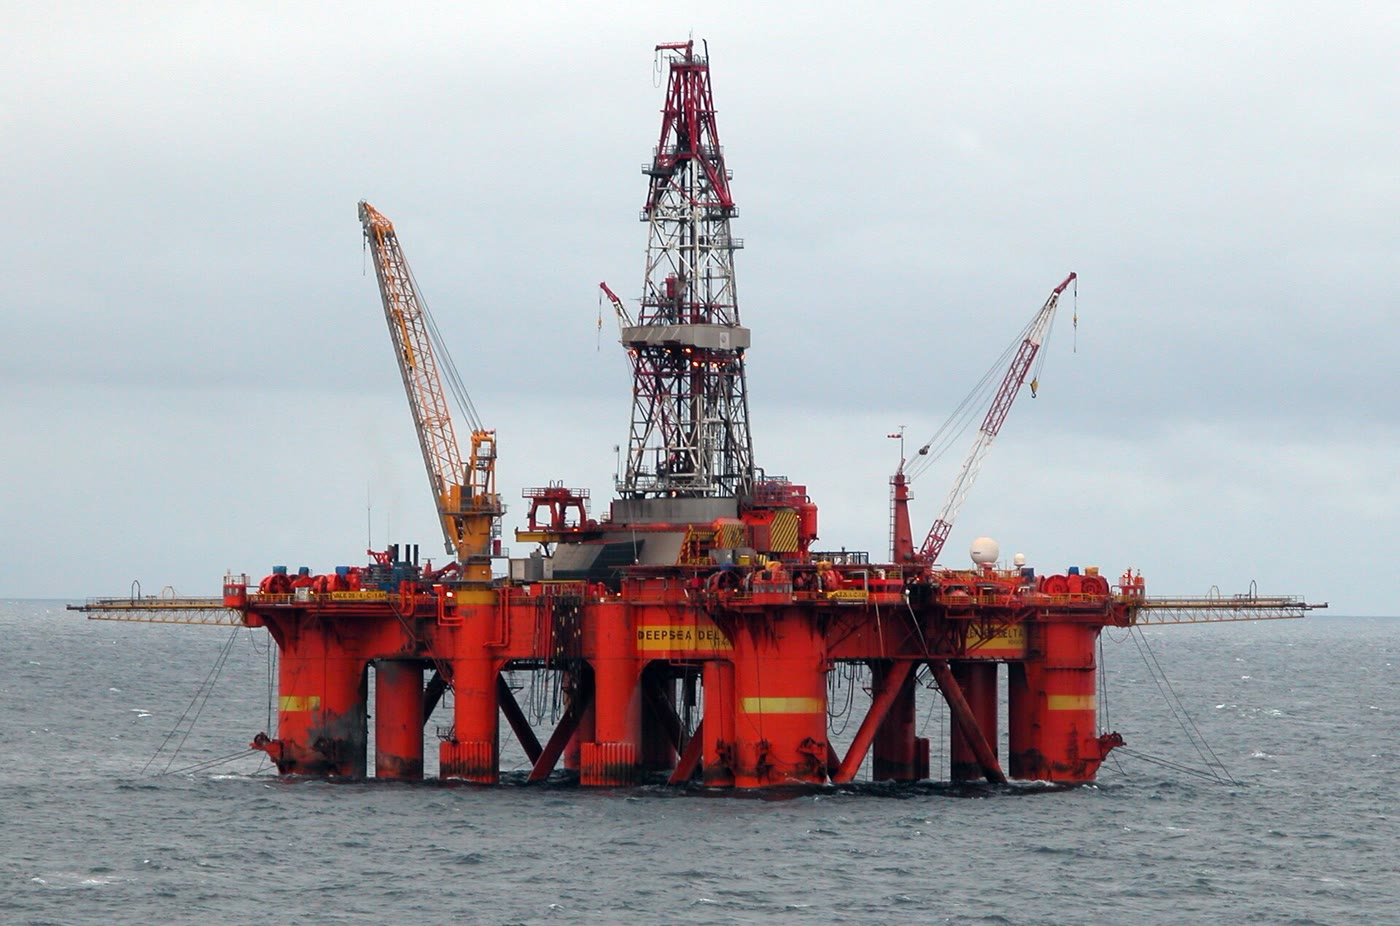
\includegraphics[width=0.66\linewidth]{images/book4/b2-16-drilling-rig.jpg}
\par\smallskip{\small Een halfafzinkbaar booreiland in de Noordzee. De boringen die
vanaf zulke eilanden worden geboord, geven de diktes, ouderdommen en gesteentesoorten waaruit de subsidentie van een bekken
wordt gereconstrueerd. Foto Erik Christensen, 2005, CC BY-SA 3.0.}
\end{omfigure}

\section{Bekkens en wat ze doet dalen}\label{sec:b2:basins-compared:types}

Boek~3 onderscheidde bekkens naar de plaats waar ze liggen. Hier worden ze onderscheiden naar wat
hun subsidentie aandrijft.

\begin{definition}[Intracratonische bekkens, riftbekkens en bekkens van passieve randen]\label{def:b2:basins-compared:types}
Een \emph{intracratonisch bekken}\index{intracratonisch bekken} is een breed, rond of ovaal bekken in het
binnenland van een continent, ver van plaatgrenzen, dat over zeer lange tijden langzaam daalt
zonder grote breukvorming. Een \emph{riftbekken}\index{riftbekken} is een bekken begrensd door afschuivingen
in een continentale lithosfeer die wordt uitgerekt; zijn subsidentie volgt de rek en daarna
de afkoeling van de lithosfeer. Een \emph{bekken van een passieve rand}\index{bekken van een passieve rand} is de
sedimentwig, zeewaarts dikker wordend, die zich na het opbreken op een continentale rand ophoopt,
boven de verdunde korst van de oude rift.
\end{definition}

Het \omterm{def:b2:alpine-orogen:foreland}{voorlandbekken} van \cref{ch:b2:alpine-orogen} maakt de lijst compleet, en de bekkens die
langs horizontale verschuivingen opengaan, worden aan Boek~5 overgelaten. Drie mechanismen doen de bodem van een
bekken dalen:
\begin{itemize}
  \item \emph{mechanische} verdunning: wanneer de korst door breuken wordt uitgerekt en verdund, wordt lichte
        korst vervangen door dichtere mantel en daalt het oppervlak om de isostasie te herstellen;
  \item \emph{thermische} contractie: een lithosfeer die is verhit, door rek of van
        onderen, koelt daarna af, wordt dichter en daalt, langzaam, over tientallen miljoenen jaren;
  \item \emph{belasting}: het gewicht van een overschuivingsgordel, of van het sediment zelf, buigt de
        lithosfeer omlaag; die flexuur hoort bij Boek~5, en de lokale, Airy-vorm van
        de sedimentlast volstaat hier.
\end{itemize}
\omterm{def:b2:basins-compared:types}{Riftbekkens} combineren de eerste twee, passieve randen erven de tweede van hun riftstadium,
\omterm{def:b2:alpine-orogen:foreland}{voorlandbekkens} worden door de derde gemaakt. \omterm{def:b2:basins-compared:types}{Intracratonische bekkens} worden het minst begrepen.

\begin{omfigure}
\centering
\begin{tikzpicture}[x=1cm, y=1cm, font=\scriptsize, line join=round,
  sed/.style={fill=yellow!35, draw=black!60, line width=0.3pt},
  crust/.style={fill=orange!25, draw=black!60, line width=0.3pt},
  mlith/.style={fill=green!12, draw=black!60, line width=0.3pt},
  asth/.style={fill=red!12, draw=black!60, line width=0.3pt},
  sea/.style={fill=blue!8, draw=none},
  ttl/.style={anchor=south west, font=\scriptsize\bfseries}]
% (a) intracratonic
\begin{scope}
\fill[asth] (0,-2.4) rectangle (6.6,-1.6);
\fill[mlith] (0,-1.6) rectangle (6.6,-0.7);
\fill[crust] (0,-0.7) -- (6.6,-0.7) -- (6.6,0) -- (4.9,0) .. controls (4.1,-0.45) and (2.5,-0.45) .. (1.7,0) -- (0,0) -- cycle;
\fill[sed] (1.7,0) .. controls (2.5,-0.45) and (4.1,-0.45) .. (4.9,0) -- cycle;
\draw[black!70] (0,0) -- (6.6,0);
\node[ttl] at (0,0.05) {(a) intracratonisch};
\node at (3.3,-1.15) {mantellithosfeer};
\node at (3.3,-2.0) {asthenosfeer};
\end{scope}
% (b) rift
\begin{scope}[xshift=7.2cm]
\fill[asth] (0,-2.4) -- (6.6,-2.4) -- (6.6,-1.6) -- (4.5,-1.6) -- (3.3,-1.0) -- (2.1,-1.6) -- (0,-1.6) -- cycle;
\fill[mlith] (0,-1.6) -- (2.1,-1.6) -- (3.3,-1.0) -- (4.5,-1.6) -- (6.6,-1.6) -- (6.6,-0.7) -- (4.4,-0.7) -- (3.3,-0.45) -- (2.2,-0.7) -- (0,-0.7) -- cycle;
\fill[crust] (0,-0.7) -- (2.2,-0.7) -- (3.3,-0.45) -- (4.4,-0.7) -- (6.6,-0.7) -- (6.6,0) -- (4.6,0) -- (4.25,-0.42) -- (3.75,-0.2) -- (3.35,-0.4) -- (2.95,-0.15) -- (2.45,-0.42) -- (2.0,0) -- (0,0) -- cycle;
\fill[sed] (2.0,0) -- (2.45,-0.42) -- (2.95,-0.15) -- (3.35,-0.4) -- (3.75,-0.2) -- (4.25,-0.42) -- (4.6,0) -- cycle;
\draw[thick] (2.0,0) -- (2.5,-0.5) (4.6,0) -- (4.2,-0.5) (2.95,-0.15) -- (3.4,-0.48);
\draw[black!70] (0,0) -- (6.6,0);
\node[ttl] at (0,0.05) {(b) rift};
\node at (1.45,-1.15) {mantellithosfeer};
\node at (5.4,-2.0) {asthenosfeer};
\end{scope}
% (c) passive margin
\begin{scope}[yshift=-3.3cm]
\fill[asth] (0,-2.4) -- (6.6,-2.4) -- (6.6,-1.2) -- (0,-1.6) -- cycle;
\fill[mlith] (0,-1.6) -- (6.6,-1.2) -- (6.6,-1.0) -- (4.2,-1.05) -- (2.4,-0.75) -- (0,-0.7) -- cycle;
\fill[crust] (0,-0.7) -- (2.4,-0.75) -- (4.2,-1.05) -- (4.2,-0.85) -- (2.6,-0.25) -- (1.6,0) -- (0,0) -- cycle;
\fill[gray!35, draw=black!60, line width=0.3pt] (4.2,-1.05) -- (6.6,-1.0) -- (6.6,-0.85) -- (4.2,-0.85) -- cycle;
\fill[sed] (1.6,0) -- (2.6,-0.25) -- (4.2,-0.85) -- (6.6,-0.85) -- (6.6,-0.55) -- (3.6,-0.45) -- (2.6,-0.05) -- (2.2,0) -- cycle;
\fill[sea] (2.2,0) -- (6.6,0) -- (6.6,-0.55) -- (3.6,-0.45) -- (2.6,-0.05) -- cycle;
\draw[black!70] (0,0) -- (2.2,0);
\draw[blue!60!black] (2.2,0) -- (6.6,0);
\node[ttl] at (0,0.05) {(c) passieve rand};
\node at (5.4,-0.95) {\tiny oceanische korst};
\node at (1.3,-2.0) {asthenosfeer};
\node at (1.3,-1.05) {mantellithosfeer};
\end{scope}
% (d) foreland
\begin{scope}[xshift=7.2cm, yshift=-3.3cm]
\fill[asth] (0,-2.4) -- (6.6,-2.4) -- (6.6,-2.0) -- (0,-1.5) -- cycle;
\fill[mlith] (0,-1.5) -- (6.6,-2.0) -- (6.6,-1.2) -- (0,-0.7) -- cycle;
\fill[crust] (0,-0.7) -- (6.6,-1.2) -- (6.6,-0.55) -- (3.6,-0.4) .. controls (2.0,-0.15) .. (0,0) -- cycle;
\fill[sed] (0,0) .. controls (2.0,-0.15) .. (3.6,-0.4) -- (6.6,-0.55) -- (5.0,0) -- cycle;
\fill[crust, fill=orange!45] (5.0,0) -- (6.6,-0.55) -- (6.6,0.6) -- (6.1,0.6) -- cycle;
\draw[thrust fault] (6.6,-0.55) -- (5.0,0);
\draw[black!70] (0,0) -- (5.0,0);
\node[ttl] at (0,0.05) {(d) voorland};
\node[anchor=north east, font=\tiny] at (6.55,0.55) {gordel};
\node at (2.2,-1.25) {mantellithosfeer};
\node at (1.5,-2.05) {asthenosfeer};
\end{scope}
\end{tikzpicture}
\par\smallskip{\small Vier families van bekkens in schematische doorsneden door de lithosfeer (niet
op schaal; sediment in geel, continentale korst in oranje, oceanische korst in grijs). De verticale
overdrijving is groot: echte bekkens zijn honderden kilometers breed en enkele tot vijftien
kilometer diep.}
\end{omfigure}

De \omterm{def:b2:basins-compared:types}{riftbekkens} van de Noordzee zijn het klassieke geval van de eerste twee mechanismen. Er ontstonden
slenken vanaf het Trias, en de laatste grote rekfase duurde van het Midden-Jura
tot het midden van het Krijt; daarna vielen de breuken stil, en het midden van het bekken bleef dalen
als een brede schotel, gevuld met krijtkalk, zandsteen en, gedurende het grootste deel van het Tertiair, schalie en
moddersteen. Alleen met water belast, zou zijn sokkel na het stoppen van de breukvorming nog 1100 tot
\qty{1400}{m} zijn gedaald in het midden en 600 tot \qty{700}{m} op de flanken.
% ledger: sc80b4:north-sea

De passieve rand van het oosten van de Verenigde Staten toont dezelfde daling op grotere schaal.
Seismische profielen over het plat tonen meer dan \qty{14}{km} mesozoïsch en jonger gesteente in
de Baltimore Canyon Trough en \qty{8}{km} in het bekken van Georges Bank, in eenheden die
zeewaarts dikker worden. Zijn Jurassische depocentra volgen de structuren van de rift en de zones van zijn
latere thermische subsidentie.
% ledger: schlee76:atlantic, lang24:atlantic

Het Michiganbekken is het type van de \omterm{def:b2:basins-compared:types}{intracratonische bekkens}. Ovaal, enkele honderdduizenden
vierkante kilometer groot, bevat het meer dan \qty{4}{km} fanerozoïsch sediment, afgezet
in afzonderlijke episoden over zo'n 500 miljoen jaar, met weinig breukvorming. Zijn episoden van snellere
subsidentie vallen samen met die van andere bekkens in het binnenland van Noord-Amerika en van andere
continenten, wat op een oorzaak wijst die groter is dan één bekken. \omterm{def:b2:basins-compared:backstripping}{Backstripping} van meer dan 57\,000
boorgatlogs toont een langlevend, bijna cirkelvormig subsidentiepatroon, dat volgens de auteurs
door neerwaartse mantelstroming zou kunnen worden verklaard, onderbroken op de tijdstippen van twee orogenesen aan de verre
rand van het continent. Waarom \omterm{def:b2:basins-compared:types}{intracratonische bekkens} dalen, staat nog ter discussie.
% ledger: sloss82:michigan, crowe09:michigan

\section{Subsidentiecurven}\label{sec:b2:basins-compared:curves}

Een boring, of een opgemeten profiel, geeft voor elke eenheid haar huidige diepte, haar gesteentesoort en haar ouderdom,
afgelezen uit fossielen of uit correlatie. Met de waterdiepte waarin elke eenheid werd
afgezet, afgelezen uit haar fossielen en sedimentaire structuren, geeft ze de geschiedenis van het bekken.

\begin{definition}[Subsidentiecurve]\label{def:b2:basins-compared:curve}
Een \emph{subsidentiecurve}\index{subsidentiecurve} van een bekken op een plaats is de grafiek van de diepte
van een referentievlak, meestal de sokkel of de basis van de oudste eenheid, onder zeeniveau,
tegen de tijd. De \emph{totale} subsidentiecurve gebruikt de sedimentdikte zoals die op elk
tijdstip was, plus de waterdiepte; de \emph{tektonische} subsidentiecurve vervangt het sediment door water
en verwijdert zijn isostatisch effect.
\end{definition}

Een eenheid was in het verleden nooit zo dik als vandaag. Begraven verloor ze porositeit; haar korrels zijn
niet veranderd, maar haar water is eruit geperst. Boek~3 schreef de porositeit op diepte
$z$ als de wet van Athy, $\phi(z) = \phi_0\,e^{-z/c}$, en vond de vaste dikte van een laag tussen
$z_1$ en $z_2$,
\[
  T_s = (z_2 - z_1) - \phi_0 c\left(e^{-z_1/c} - e^{-z_2/c}\right),
\]
die dezelfde blijft wanneer de laag zich verplaatst. Om een eenheid te \emph{decompacteren} naar een ondiepere positie,
met haar top nu op $z_1'$, zoekt men de basis $z_2'$ die dezelfde vaste dikte bevat. De
vergelijking heeft geen gesloten oplossing, maar de vastepuntiteratie
\[
  z_2' \leftarrow z_1' + T_s + \phi_0 c\left(e^{-z_1'/c} - e^{-z_2'/c}\right)
\]
convergeert vanaf $z_2' = z_1' + T_s$ in enkele stappen. De massa per oppervlakte-eenheid van de laag
is die van haar korrels plus die van haar poriewater,
\[
  m = \rho_g T_s + \rho_w\,(z_2 - z_1 - T_s),
\]
met $\rho_g$ de dichtheid van de korrels; de massa van een kolom delen door haar dikte geeft
haar gemiddelde dichtheid $\bar\rho_s$.

Voor de lithologieën die in dit hoofdstuk worden gebruikt, zand, schalie, krijt en kleiig zand, geeft de tabel hieronder
de constanten van Sclater en Christie (1980), zoals opgenomen in een opensourceprogramma.
Zand behoudt zijn porositeit het diepst, krijt verliest ze het snelst.
% ledger: pybacktrack:compaction

\begin{center}
\small
\begin{tabular}{lccc}
\hline
lithologie & korreldichtheid (\unit{kg.m^{-3}}) & oppervlakteporositeit $\phi_0$ & vervallengte $c$ (\unit{m}) \\
\hline
zand & 2650 & 0.49 & 3704 \\
schalie & 2700 & 0.63 & 1960 \\
krijt & 2710 & 0.70 & 1408 \\
kleiig zand & 2680 & 0.56 & 2564 \\
\hline
\end{tabular}
\end{center}

\section{Backstripping}\label{sec:b2:basins-compared:backstripping}

Een totale \omterm{def:b2:basins-compared:curve}{subsidentiecurve} mengt twee oorzaken: wat het bekken ook maakte, en het gewicht van wat
het vulde. Ze scheiden is het doel van de volgende procedure, het centrale werktuig van de
bekkenanalyse.

\begin{definition}[Backstripping]\label{def:b2:basins-compared:backstripping}
\emph{Backstripping}\index{backstripping} is de reconstructie van de tektonische subsidentie van een
bekken in de loop van de tijd: de eenheden van een boring worden een voor een verwijderd, te beginnen met de jongste, de
overblijvende worden bij elke stap gedecompacteerd, en het isostatische effect van de last van sediment en water
wordt verwijderd om de diepte te geven waarop de sokkel onder alleen water zou hebben gestaan.
\end{definition}

De laatste stap is een isostatische balans. Boek~3 stelde die op voor een bekken dat tot zeeniveau is gevuld;
het algemene geval voegt de waterdiepte en het niveau van de zee toe.

\begin{proposition}[Backstripping volgens Airy]\label{prop:b2:basins-compared:backstrip}
Laat een bekken op een bepaald tijdstip een sedimentkolom bevatten met dikte $S$ en gemiddelde dichtheid
$\bar\rho_s$, onder een waterdiepte $W_d$, terwijl de zee $\Delta_{SL}$ boven haar huidige
niveau stond. In lokale isostasie boven een mantel met dichtheid $\rho_m$, met water met dichtheid $\rho_w$, is de
tektonische subsidentie op dat tijdstip, gemeten vanaf het huidige zeeniveau,
\[
  Y = S\,\frac{\rho_m - \bar\rho_s}{\rho_m - \rho_w} + W_d
      - \Delta_{SL}\,\frac{\rho_m}{\rho_m - \rho_w}.
\]
\end{proposition}

\begin{proof}
Vergelijk twee kolommen boven dezelfde lithosfeer, tot een compensatiediepte onder beide. In
de eerste ligt water met diepte $W_d$ boven het sediment met dikte $S$; in de tweede vult alleen water
een bekken met diepte $Y'$ onder hetzelfde zeeoppervlak. Hun massa's zijn gelijk:
\[
  \rho_w W_d + \bar\rho_s S + \rho_m\,(d - W_d - S) = \rho_w Y' + \rho_m\,(d - Y'),
\]
met $d$ de gemeenschappelijke diepte van het compensatieniveau onder het zeeoppervlak. Dus
$Y'(\rho_m - \rho_w) = S(\rho_m - \bar\rho_s) + W_d(\rho_m - \rho_w)$, wat de eerste twee
termen zijn. Als de zee $\Delta_{SL}$ hoger stond dan vandaag, hoort dat extra water niet bij de
eigen subsidentie van het bekken: als men het verwijdert, rijst de met water belaste sokkel met
$\Delta_{SL}\rho_w/(\rho_m - \rho_w)$, en is zijn diepte onder het huidige zeeniveau nog eens kleiner met
$\Delta_{SL}$; samen $\Delta_{SL}\,\rho_m/(\rho_m - \rho_w)$.
\end{proof}
% ledger: pybacktrack:backstrip

Met $\rho_m = \qty{3330}{kg.m^{-3}}$ en $\rho_w = \qty{1030}{kg.m^{-3}}$ telt een sedimentkolom met
gemiddelde dichtheid \qty{2300}{kg.m^{-3}} voor $1030/2300 = 0.45$ van haar dikte in de tektonische
subsidentie: meer dan de helft van de dikte van de vulling van een bekken wordt door haar eigen gewicht ingeruimd.
Een zee die \qty{100}{m} hoger staat dan vandaag, verlaagt het resultaat met \qty{145}{m}. De waterdiepte en het
vroegere zeeniveau zijn de zwakste gegevens: fossielen geven een bereik van waterdiepten, op de helling vaak honderden
meters breed, en de tektonische subsidentie erft dat bereik.

\begin{method}[Backstripping van een boring]\label{met:b2:basins-compared:backstrip}
\begin{enumerate}
  \item Som de eenheden op vanaf de basis, met de huidige diepten van hun top en basis, hun
        lithologieconstanten $(\rho_g, \phi_0, c)$, de ouderdommen van hun top, en de waterdiepte op
        elk van die ouderdommen.
  \item Bereken de vaste dikte $T_s$ van elke eenheid uit haar huidige diepten.
  \item Verwijder voor de ouderdom van de top van eenheid $k$ alle jongere eenheden. Leg de top van eenheid
        $k$ op diepte nul en decompacteer haar; leg elke oudere eenheid op haar beurt onder de eenheid erboven
        en decompacteer ze.
  \item Tel de diktes op om $S$ te krijgen, en de massa's om de gemiddelde dichtheid
        $\bar\rho_s = \sum m / S$ te krijgen.
  \item Pas \cref{prop:b2:basins-compared:backstrip} toe om $Y$ te verkrijgen; de totale subsidentie is
        $S + W_d$.
  \item Herhaal voor elke ouderdom, van de oudste tot het heden; zet $Y$ en $S + W_d$ uit tegen de ouderdom.
\end{enumerate}
\end{method}

De figuur hieronder toont het resultaat voor een verzonnen boring in een \omterm{def:b2:basins-compared:types}{riftbekken}. Er werden vier eenheden gekernd:
een synrift-zand, afgezet terwijl breuken actief waren, tussen 165 en \qty{150}{Ma}; daarna een schalie,
een krijt en een kleiig zand. Vandaag is er geen decompactie nodig: de sokkel ligt op \qty{6030}{m}
en de kolom heeft een gemiddelde dichtheid van \qty{2358}{kg.m^{-3}}, zodat $Y = \qty{2648}{m}$ onder
\qty{100}{m} water. Op \qty{150}{Ma} was het zand alleen, aan het oppervlak gedecompacteerd,
\qty{2239}{m} dik, met een gemiddelde dichtheid van \qty{2055}{kg.m^{-3}}: onder \qty{200}{m} water was
$Y = \qty{1441}{m}$. De totale subsidentie is
meer dan tweemaal de tektonische, en de tektonische curve toont een snel eerste stadium, daarna een
vertragende daling: de vorm van een rift.
% values (script): figdata/bachelor-2/basins.py part numbers (S_150 2239.5, rho_0 2357.9, Y_0 2648.7, Y_150 1442.1); printed from the rounded chain of calc/ch16.py (rho 2358 -> 2648; T 2239, rho 2055 -> 1441), as in the problem

\begin{omfigure}
\centering
% figdata/bachelor-2/basins.py parts stages and fit (invented well)
\begin{tikzpicture}
\begin{axis}[width=0.8\linewidth, height=6.0cm, x dir=reverse, y dir=reverse, xmin=0, xmax=170,
  ymin=0, ymax=6500, xlabel={ouderdom (\unit{Ma})}, ylabel={diepte onder zeeniveau (\unit{m})},
  tick label style={font=\scriptsize}, label style={font=\small}, xtick={0,25,...,175},
  xtick pos=bottom, ytick pos=left,
  legend style={at={(0.5,1.04)}, anchor=south, draw=none, font=\scriptsize, legend columns=3,
  /tikz/every even column/.append style={column sep=8pt}}]
\addplot[omThm, line width=1pt, mark=*, mark size=1.6pt] table[x=age_Ma, y=total_m]
  {figdata/out/bachelor-2-basins-stages.dat};
\addlegendentry{totale subsidentie $S + W_d$}
\addplot[blue!70!black, line width=1pt, mark=square*, mark size=1.6pt] table[x=age_Ma, y=Y_m]
  {figdata/out/bachelor-2-basins-stages.dat};
\addlegendentry{tektonische subsidentie $Y$}
\addplot[black!70, dashed, line width=0.8pt] table[x=age_Ma, y=Y_m]
  {figdata/out/bachelor-2-basins-fit.dat};
\addlegendentry{rekmodel, $\beta = 1.50$}
\node[font=\scriptsize, anchor=south west] at (axis cs:149,1500) {einde van de riftvorming};
\end{axis}
\end{tikzpicture}
\par\smallskip{\small \omterm{def:b2:basins-compared:backstripping}{Backstripping} van een verzonnen boring met vier eenheden (gegevens in het
weekendprobleem): diepte van de sokkel met het sediment zoals het op elk tijdstip was, en tektonische subsidentie,
met de curve van het \omterm{def:b2:basins-compared:stretching}{rekmodel} aangepast aan de subsidentie aan het eind van de riftvorming
(\cref{sec:b2:basins-compared:stretching}).}
\end{omfigure}

\begin{omfigure}
\centering
\begin{tikzpicture}[x=1cm, y=0.1cm, font=\scriptsize, line join=round,
  u/.style={draw=black!60, line width=0.3pt}]
% today
\begin{scope}
\fill[blue!8] (0,0) rectangle (1.6,-1.0);
\fill[u, fill=yellow!25] (0,-1.0) rectangle (1.6,-18.0);
\fill[u, fill=green!18] (0,-18.0) rectangle (1.6,-34.1);
\fill[u, fill=gray!25] (0,-34.1) rectangle (1.6,-45.2);
\fill[u, fill=yellow!55] (0,-45.2) rectangle (1.6,-61.3);
\draw[black!70] (0,-61.3) -- (1.6,-61.3);
\node[anchor=south] at (0.8,0.1) {vandaag};
\node at (0.8,-9.5) {kleiig zand};
\node at (0.8,-26) {krijt};
\node at (0.8,-39.6) {schalie};
\node at (0.8,-53.2) {zand};
\node[anchor=north] at (0.8,-61.5) {\qty{6130}{m}};
\end{scope}
% at 150 Ma
\begin{scope}[xshift=3.0cm]
\fill[blue!8] (0,0) rectangle (1.6,-2.0);
\fill[u, fill=yellow!55] (0,-2.0) rectangle (1.6,-24.39);
\draw[black!70] (0,-24.4) -- (1.6,-24.4);
\node[anchor=south] at (0.8,0.1) {\qty{150}{Ma}};
\node at (0.8,-13.2) {zand};
\node[anchor=north] at (0.8,-24.6) {\qty{2439}{m}};
\end{scope}
\draw[-{Latex}, thick] (4.9,-12) -- (6.1,-12) node[midway, above] {ontlasten};
% water loaded
\begin{scope}[xshift=6.3cm]
\fill[blue!20] (0,0) rectangle (1.6,-14.4);
\draw[black!70] (0,-14.4) -- (1.6,-14.4);
\node[anchor=south] at (0.8,0.1) {alleen water};
\node at (0.8,-7.2) {water};
\node[anchor=north] at (0.8,-14.6) {$Y = \qty{1441}{m}$};
\end{scope}
\draw[black!40, dashed] (-0.3,0) -- (8.2,0);
\node[anchor=west] at (8.2,0) {zeeniveau};
\end{tikzpicture}
\par\smallskip{\small \omterm{def:b2:basins-compared:backstripping}{Backstripping} van de verzonnen boring op \qty{150}{Ma} (diepten op schaal): de
vier eenheden vandaag; het zand alleen aan het eind van de riftvorming, aan het oppervlak gedecompacteerd onder
\qty{200}{m} water; dezelfde lithosfeer alleen met water belast, waarvan de sokkel
hoger staat omdat water lichter is dan sediment.}
\end{omfigure}

\section{Het rekmodel}\label{sec:b2:basins-compared:stretching}

Waarom daalt een \omterm{def:b2:basins-compared:types}{riftbekken} eerst snel en daarna langzaam? In 1978 stelde D. McKenzie een model voor dat zo
eenvoudig is dat zijn parameters aan één boring kunnen worden aangepast.

\begin{definition}[Rekmodel; rekfactor; synrift- en postrift-subsidentie]\label{def:b2:basins-compared:stretching}
Het \emph{rekmodel}\index{rekmodel} van een bekken stelt riftvorming voor als een
ogenblikkelijke, uniforme rek van de hele lithosfeer door zuivere schuif: korst en
mantellithosfeer worden met dezelfde factor verdund, en hete asthenosfeer stijgt passief op om de
ruimte te vullen, waarna de lithosfeer afkoelt. De \emph{rekfactor}\index{rekfactor}
$\beta$ is de verhouding van de breedte van het uitgerekte gebied na de rek tot zijn breedte ervoor,
gelijk aan de verhouding van de begin- tot de einddikte van de korst. De subsidentie die
tijdens de rek ontstaat, is de \emph{synrift-subsidentie}\index{synrift-subsidentie}; die welke
daarna door de afkoeling van de lithosfeer ontstaat, is de
\emph{postrift-subsidentie}\index{postrift-subsidentie}, of thermische subsidentie.
\end{definition}

Rek in de natuur neemt een eindige tijd in beslag, miljoenen jaren. Latere versies van het model laten haar
duren, maar zolang ze niet te traag is, geeft de eenvoudige ogenblikkelijke versie de subsidentie
ruw maar correct, omdat de afkoeling na de rek grotendeels op dezelfde manier verloopt.
% ledger: sheplev98:model

\begin{omfigure}
\centering
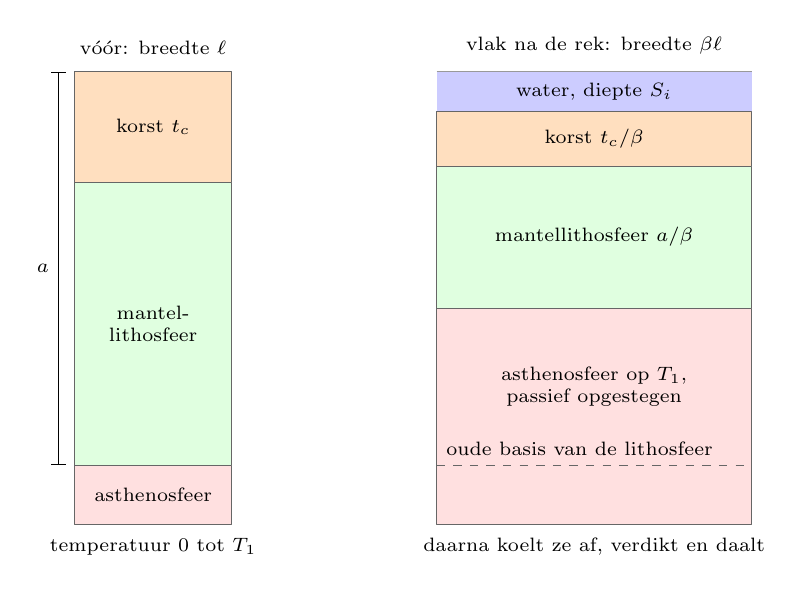
\begin{tikzpicture}[x=0.5cm, y=0.5cm, font=\scriptsize, line join=round]
% before
\begin{scope}
\fill[orange!25, draw=black!60, line width=0.3pt] (0,0) rectangle (4,-2.8);
\fill[green!12, draw=black!60, line width=0.3pt] (0,-2.8) rectangle (4,-10);
\fill[red!12, draw=black!60, line width=0.3pt] (0,-10) rectangle (4,-11.5);
\node at (2,-1.4) {korst $t_c$};
\node[align=center] at (2,-6.4) {mantel-\\lithosfeer};
\node at (2,-10.75) {asthenosfeer};
\draw[|-|] (-0.4,0) -- (-0.4,-10) node[midway, left] {$a$};
\node[anchor=south] at (2,0.2) {vóór: breedte $\ell$};
\node[anchor=north] at (2,-11.6) {temperatuur $0$ tot $T_1$};
\end{scope}
% after
\begin{scope}[xshift=4.6cm]
\fill[blue!20] (0,0) rectangle (8,-1.0);
\fill[orange!25, draw=black!60, line width=0.3pt] (0,-1.0) rectangle (8,-2.4);
\fill[green!12, draw=black!60, line width=0.3pt] (0,-2.4) rectangle (8,-6.0);
\fill[red!12, draw=black!60, line width=0.3pt] (0,-6.0) rectangle (8,-11.5);
\draw[black!60, dashed] (0,-10) -- (8,-10);
\node at (4,-0.5) {water, diepte $S_i$};
\node at (4,-1.7) {korst $t_c/\beta$};
\node at (4,-4.2) {mantellithosfeer $a/\beta$};
\node[align=center] at (4,-8.0) {asthenosfeer op $T_1$,\\passief opgestegen};
\node[anchor=south west] at (0,-10) {oude basis van de lithosfeer};
\node[anchor=south] at (4,0.2) {vlak na de rek: breedte $\beta\ell$};
\node[anchor=north] at (4,-11.6) {daarna koelt ze af, verdikt en daalt};
\draw[black!40] (0,0) -- (8,0);
\end{scope}
\end{tikzpicture}
\par\smallskip{\small Het \omterm{def:b2:basins-compared:stretching}{rekmodel} (niet op schaal): een lithosfeer met dikte $a$ en een
korst $t_c$ wordt uitgerekt tot $\beta$ keer haar breedte; korst en mantellithosfeer worden dunner met
$\beta$, de asthenosfeer stijgt op, en het oppervlak daalt met de \omterm{def:b2:basins-compared:stretching}{synrift-subsidentie} $S_i$ onder
water. Hier is $\beta = 2$.}
\end{omfigure}

\begin{proposition}[Subsidentie in het rekmodel]\label{prop:b2:basins-compared:stretching}
Laat een lithosfeer met dikte $a$ en een korst met dikte $t_c$ een lineaire geotherm hebben van
$0$ aan het oppervlak tot de temperatuur $T_1$ van de asthenosfeer aan haar basis; laat korst en mantel
dichtheden $\rho_c(1 - \alpha T)$ en $\rho_m(1 - \alpha T)$ hebben, met $\alpha$ de thermische
uitzettingscoëfficiënt. Als ze ogenblikkelijk wordt uitgerekt met $\beta$ en het bekken met
water met dichtheid $\rho_w$ wordt gevuld, dan geldt:
\begin{enumerate}
  \item de \omterm{def:b2:basins-compared:stretching}{synrift-subsidentie} is
  \[
    S_i = \frac{a\left(1 - \dfrac{1}{\beta}\right)\left[(\rho_m - \rho_c)\dfrac{t_c}{a}
          \left(1 - \dfrac{\alpha T_1 t_c}{2a}\right) - \dfrac{\alpha T_1 \rho_m}{2}\right]}
          {\rho_m(1 - \alpha T_1) - \rho_w};
  \]
  \item de \omterm{def:b2:basins-compared:stretching}{postrift-subsidentie}, een tijd $t$ na de rek, is, tot op de eerste term van een reeks,
  \[
    S_t = E_0\,\frac{\beta}{\pi}\sin\frac{\pi}{\beta}\left(1 - e^{-t/\tau}\right),\qquad
    E_0 = \frac{4a\rho_m\alpha T_1}{\pi^2(\rho_m - \rho_w)},\qquad
    \tau = \frac{a^2}{\pi^2\kappa},
  \]
  waarbij $\kappa$ de thermische diffusiviteit is en $\tau$ de \emph{thermische
tijdconstante}\index{thermische tijdconstante} van de lithosfeer.
\end{enumerate}
\end{proposition}
% ledger: pybacktrack:rifting

\begin{proof}
(1) Vergelijk de kolom vóór de rek met de kolom vlak erna, tot de oude basis van
de lithosfeer, op diepte $a$ onder het oppervlak vóór de rek. Ervoor staan de korst met
dikte $t_c$ en de mantellithosfeer op temperaturen $T = T_1 z/a$; erna zijn beide
dunner met $\beta$ en lopen hun temperaturen van $0$ tot $T_1$ over $a/\beta$, zodat een punt
op diepte $z'$ onder de basis van het water $T = T_1\beta z'/a$ heeft; eronder heeft de asthenosfeer op
$T_1$ de dichtheid $\rho_m(1 - \alpha T_1)$; erboven vult water de diepte $S_i$. De massa van een
laag met dichtheid $\rho(1 - \alpha T)$ waarin $T$ lineair groeit van $T_a$ tot $T_b$, is
$\rho\,h\,(1 - \alpha(T_a + T_b)/2)$. Ervoor bevat de kolom
\[
  \rho_c t_c\left(1 - \frac{\alpha T_1 t_c}{2a}\right)
  + \rho_m (a - t_c)\left(1 - \frac{\alpha T_1 (a + t_c)}{2a}\right);
\]
erna bevat ze het water, de verdunde korst en mantellithosfeer, en de asthenosfeer die
de rest van de diepte $a$ vult:
\[
  \rho_w S_i + \frac{\rho_c t_c}{\beta}\left(1 - \frac{\alpha T_1 t_c}{2a}\right)
  + \frac{\rho_m (a - t_c)}{\beta}\left(1 - \frac{\alpha T_1 (a + t_c)}{2a}\right)
  + \rho_m(1 - \alpha T_1)\left(a - S_i - \frac{a}{\beta}\right).
\]
Isostasie maakt de twee gelijk. De termen in $S_i$ aan de ene kant en de factor
$(1 - 1/\beta)$ aan de andere kant samenbrengen en uitwerken geeft de formule; de algebra is
\cref{exo:b2:basins-compared:11}.

(2) Na de rek koelt de plaat af door geleiding tussen een oppervlak op $0$ en een basis op
$T_1$, naar het lineaire profiel waarvan ze uitging. De overtemperatuur lost de
warmtevergelijking op met nulwaarden aan top en basis, en is dus een som van termen
$b_n\sin(n\pi z/a)\,e^{-n^2\kappa\pi^2 t/a^2}$; elke term koelt af met zijn eigen tijd, $\tau/n^2$. Het
warmteverlies doet de kolom inkrimpen met $\alpha\int \Delta T\,\mathrm{d}z$, en het extra water
dat de ruimte vult, doet haar verder dalen met de factor $\rho_m/(\rho_m - \rho_w)$. Alleen oneven termen
dragen bij; de eerste behouden, waarvan de coëfficiënt uit het beginprofiel wordt berekend, geeft
de uitdrukking. De andere koelen negen of meer keer sneller af, en na ongeveer tien miljoen jaar
verschuiven ze de subsidentie met een bijna constant bedrag, minder dan \qty{100}{m} voor $\beta$ van
1.2 tot 4 met de waarden hieronder.
\end{proof}
% values (script): basins.thermal_series vs basins.thermal, tested in tests/bachelor-2/test_basins.py

De parameters van het artikel van McKenzie zijn $a = \qty{125}{km}$, $T_1 = \qty{1333}{\celsius}$,
$\alpha = \qty{3.28e-5}{K^{-1}}$, $\kappa = \qty{8e-7}{m^2.s^{-1}}$, $\rho_m =
\qty{3330}{kg.m^{-3}}$ (bij \qty{0}{\celsius}), $\rho_c = \qty{2800}{kg.m^{-3}}$; met zeewater van
\qty{1030}{kg.m^{-3}} geven ze $\tau = \qty{62.7}{Myr}$ en $E_0 = \qty{3207}{m}$. Met een korst van
\qty{35}{km} is de \omterm{def:b2:basins-compared:stretching}{synrift-subsidentie} $S_i = \qty{4334}{m} \times (1 - 1/\beta)$.
% ledger: sheplev98:parameters, pybacktrack:rifting
% values (script): tau_Myr 62.7, E0_m 3206.9, Si_max_m 4333.8

\begin{omfigure}
\centering
% figdata/bachelor-2/basins.py part curves
\begin{tikzpicture}
\begin{axis}[width=0.8\linewidth, height=6.2cm, y dir=reverse, xmin=0, xmax=200, ymin=0,
  ymax=6500, xlabel={tijd na de rek (\unit{Myr})},
  ylabel={tektonische subsidentie (\unit{m})}, tick label style={font=\scriptsize},
  label style={font=\small}, xtick pos=bottom, ytick pos=left]
\addplot[black!45, line width=1pt] table[x=t_Myr, y=b1.2] {figdata/out/bachelor-2-basins-curves.dat};
\addplot[blue!70!black, line width=1pt] table[x=t_Myr, y=b1.5] {figdata/out/bachelor-2-basins-curves.dat};
\addplot[omThm, line width=1pt] table[x=t_Myr, y=b2] {figdata/out/bachelor-2-basins-curves.dat};
\addplot[orange!80!black, line width=1pt] table[x=t_Myr, y=b4] {figdata/out/bachelor-2-basins-curves.dat};
\node[font=\scriptsize, anchor=south west, inner sep=1pt] at (axis cs:150,1225) {$\beta = 1.2$};
\node[font=\scriptsize, anchor=south west, inner sep=1pt] at (axis cs:150,2595) {$\beta = 1.5$};
\node[font=\scriptsize, anchor=south west, inner sep=1pt] at (axis cs:150,3965) {$\beta = 2$};
\node[font=\scriptsize, anchor=south west, inner sep=1pt] at (axis cs:150,5815) {$\beta = 4$};
\draw[black!40, dashed] (axis cs:62.7,0) -- (axis cs:62.7,6500);
\node[font=\scriptsize, anchor=north west] at (axis cs:63,150) {$t = \tau$};
\end{axis}
\end{tikzpicture}
\par\smallskip{\small Met water belaste subsidentie van het \omterm{def:b2:basins-compared:stretching}{rekmodel} voor vier
\omterm{def:b2:basins-compared:stretching}{rekfactoren}, met een korst van \qty{35}{km} en de parameters van de tekst: de synrift-stap op
$t = 0$, daarna de postrift-curve, die op $t = \tau$ \qty{63}{\percent} van haar eindwaarde heeft
bereikt.}
\end{omfigure}

Drie kenmerken van het model gaan over op echte bekkens.
\begin{itemize}
  \item De synrift-stap groeit met $\beta$, en de \omterm{def:b2:basins-compared:stretching}{postrift-subsidentie} ook; maar hun
        verhouding verandert weinig, zodat beide delen naar dezelfde $\beta$ wijzen als het model klopt.
  \item De tijdschaal van de \omterm{def:b2:basins-compared:stretching}{postrift-subsidentie} hangt niet af van $\beta$: ze wordt bepaald door de
        dikte van de lithosfeer alleen. Na $\tau$ is \qty{63}{\percent} van de thermische
        subsidentie voltooid; na $3\tau$ ongeveer \qty{95}{\percent}. Een rift die tweehonderd
        miljoen jaar geleden stopte, daalt nauwelijks nog.
  \item De synrift-term is een wedstrijd tussen de verdunde lichte korst, die het
        oppervlak doet dalen, en de opgestegen hete asthenosfeer, die het opdrijft. Met een dunne korst wint de
        tweede en heft de rek het oppervlak op (\cref{exo:b2:basins-compared:10}).
\end{itemize}

Om een boring aan te passen, geeft de tektonische subsidentie aan het eind van de riftvorming $S_i$, dus
$\beta = 1/(1 - S_i/\qty{4334}{m})$ voor een korst van \qty{35}{km}; de postrift-curve wordt dan voorspeld
en vergeleken met de rest van de gebackstripte punten. In de verzonnen boring geeft $S_i = \qty{1441}{m}$
$\beta = 1.50$, en de curve loopt op enkele meters na door de latere punten (figuur in
\cref{sec:b2:basins-compared:backstripping}). Echte bekkens zijn zelden zo meegaand. In de
centrale Noordzee reproduceert een rek van 50 tot \qty{100}{\percent} in het midden, $\beta$ van 1.5 tot 2,
de amplitude en de snelheid van de \omterm{def:b2:basins-compared:stretching}{postrift-subsidentie}. Op de rand van het oosten van de Verenigde
Staten heeft slechts één segment, het Long Island Platform, een vroege postrift-vulling die zo dik is
als uniforme rek voorspelt; in het bekken van Georges Bank en de Baltimore Canyon Trough is de
vulling 1.5 tot 3 keer dikker, en moeten andere oorzaken werkzaam zijn.
% ledger: sc80b4:north-sea, lang24:atlantic

\section{Bekkens vergeleken}\label{sec:b2:basins-compared:compared}

De tabel hieronder brengt de vier families samen. De curven verschillen in vorm en in tijdschaal, en een
\omterm{def:b2:basins-compared:curve}{subsidentiecurve} is vaak de eerste aanwijzing voor de aard van een bekken dat onder jongere gesteenten begraven ligt.

\begin{center}
\small
\begin{tabular}{>{\raggedright\arraybackslash}p{0.13\linewidth}>{\raggedright\arraybackslash}p{0.19\linewidth}>{\raggedright\arraybackslash}p{0.26\linewidth}>{\raggedright\arraybackslash}p{0.29\linewidth}}
\hline
bekken & voorbeeld & dikte en duur & vorm van de tektonische \omterm{def:b2:basins-compared:curve}{subsidentiecurve} \\
\hline
rift & centrale Noordzee & slenken vanaf het Trias; laatste rek van Midden-Jura tot
midden-Krijt; 1.1 tot \qty{1.4}{km} met water belaste postrift-daling & een snelle synrift-stap,
daarna een exponentiële vertraging met $\tau$ van tientallen Myr \\
passieve rand & Baltimore Canyon Trough & meer dan \qty{14}{km} sinds het Jura & zoals een
rift, met een groot postrift-deel; de vulling wordt zeewaarts dikker \\
voorland & Noord-Alpiene \omterm{def:b2:alpine-orogen:foreland}{Molasse} & meer dan \qty{4}{km} aan het overschuivingsfront, Laat-Eoceen tot
Laat-Mioceen & het diepst tegen de gordel en ermee migrerend; het binnenste deel uiteindelijk
overreden door de overschuivingen \\
\hspace{0pt}intra\-cratonisch & Michigan & meer dan \qty{4}{km} in episoden over zo'n 500 Myr & langzaam, met
episoden van snellere daling die verre bekkens delen \\
\hline
\end{tabular}
\end{center}
% ledger: sc80b4:north-sea, schlee76:atlantic, poag79:bct, krenmayr99:molasse, schmid04:foreland, sloss82:michigan

Een \omterm{def:b2:alpine-orogen:foreland}{voorlandbekken} daalt onder een last die ernaartoe beweegt: het bekken migreert met de gordel,
het Alpiene over minstens \qty{210}{km} over het Europese craton, en zijn binnenste deel wordt
uiteindelijk overreden en door de overschuivingen meegevoerd, zoals de Subalpiene \omterm{def:b2:alpine-orogen:foreland}{Molasse} in
\cref{ch:b2:alpine-orogen}. Een rift vertraagt terwijl hij afkoelt, wat
zijn rek ook is. Een \omterm{def:b2:basins-compared:types}{intracratonisch bekken} daalt langzaam en lang, met pulsen; noch rek
noch een last verklaart het goed, en daarom blijft het een onderzoeksvraag.
% ledger: schmid04:foreland, sinclair97:trinity, krenmayr99:molasse

\begin{inthelab}[Subsidentieanalyse]
Bekkenanalisten doen het werk van het methodekader met programma's. Een opensourceprogramma
leest bijvoorbeeld een boorlocatie als een lijst eenheden met hun ouderdommen, diepten en lithologieën, en een
tabel van lithologieën met hun korreldichtheid, oppervlakteporositeit en vervallengte. Zijn
backstrippingmodule decompacteert de eenheden en geeft de tektonische subsidentie op elke ouderdom terug;
omdat een vroegere waterdiepte alleen als bereik bekend is, geeft de gebruiker een minimum en een maximum en
geeft het programma de twee subsidenties en hun gemiddelde terug. Een tweede module werkt omgekeerd:
uit een model van tektonische subsidentie voorspelt het de waterdiepten van het verleden, die kunnen worden
getoetst aan de fossielen. Analisten passen daarna \omterm{def:b2:basins-compared:stretching}{rekfactoren} aan, toetsen zeespiegelcurven en
brengen de subsidentie van een heel bekken in kaart uit honderden of duizenden boringen.
\end{inthelab}
% ledger: pybacktrack:modules, crowe09:michigan

\section*{Oefeningen}\label{sec:b2:basins-compared:exercises}

Gegevens voor de oefeningen, tenzij anders vermeld: $\rho_m = \qty{3330}{kg.m^{-3}}$, $\rho_c =
\qty{2800}{kg.m^{-3}}$, $\rho_w = \qty{1030}{kg.m^{-3}}$; \omterm{def:b2:basins-compared:stretching}{rekmodel} met $a =
\qty{125}{km}$, $T_1 = \qty{1333}{\celsius}$, $\alpha = \qty{3.28e-5}{K^{-1}}$, $\kappa =
\qty{8e-7}{m^2.s^{-1}}$, $\tau = \qty{62.7}{Myr}$, $E_0 = \qty{3207}{m}$; een korst van \qty{35}{km}
geeft $S_i = \qty{4334}{m}\times(1 - 1/\beta)$; lithologieconstanten in de tabel van
\cref{sec:b2:basins-compared:curves}.

\begin{exercise}[$\star$]\label{exo:b2:basins-compared:1}
Benoem de familie van elk bekken en de belangrijkste oorzaak van zijn subsidentie: (a) het Michiganbekken;
(b) de centrale Noordzee; (c) de Baltimore Canyon Trough; (d) de Noord-Alpiene \omterm{def:b2:alpine-orogen:foreland}{Molasse};
(e) de Indo-Gangetische vlakte vóór de Himalaya.
\end{exercise}

\begin{exercise}[$\star$]\label{exo:b2:basins-compared:2}
Een bekken bevat \qty{3.0}{km} sediment met gemiddelde dichtheid \qty{2300}{kg.m^{-3}}. (a) Bepaal zijn
tektonische subsidentie als het sediment tot zeeniveau reikt. (b) En als er \qty{200}{m} water
bovenop ligt? (c) Welke fractie van de dikte van de vulling is te danken aan de last van de vulling zelf?
\end{exercise}

\begin{exercise}[$\star$]\label{exo:b2:basins-compared:3}
Seismische refractie toont dat een korst van \qty{35}{km} in een rift is verdund tot \qty{25}{km}.
(a) Wat is $\beta$? (b) Hoe dik is de lithosfeer vlak na de rek? (c) Wat is de
\omterm{def:b2:basins-compared:stretching}{synrift-subsidentie} onder water?
\end{exercise}

\begin{exercise}[$\star$]\label{exo:b2:basins-compared:4}
(a) Controleer dat $\tau = \qty{62.7}{Myr}$ ($1~\text{Myr} = \qty{3.156e13}{s}$). (b) Sommige programma's
gebruiken $\kappa = \qty{1e-6}{m^2.s^{-1}}$: wat is $\tau$ dan? (c) Wat zou ze zijn voor een
lithosfeer van \qty{100}{km} dik, met $\kappa = \qty{8e-7}{m^2.s^{-1}}$? (d) Welke fractie van
de \omterm{def:b2:basins-compared:stretching}{postrift-subsidentie} is voltooid na $\tau$, en na $3\tau$?
\end{exercise}

\begin{exercise}[$\star\star$]\label{exo:b2:basins-compared:5}
Een schalie-eenheid ligt vandaag tussen \qty{1000}{m} en \qty{2000}{m}. (a) Bepaal haar porositeit aan de
top en aan de basis. (b) Bepaal haar vaste dikte. (c) Bepaal haar massa per oppervlakte-eenheid en haar gemiddelde
dichtheid, als de poriën met water gevuld zijn.
\end{exercise}

\begin{exercise}[$\star\star$]\label{exo:b2:basins-compared:6}
De schalie van \cref{exo:b2:basins-compared:5} wordt terug naar het oppervlak gebracht. (a) Itereer de
decompactieformule vanaf $z_2' = T_s$ tot ze minder dan \qty{1}{m} verandert. (b) Wat is
haar gemiddelde dichtheid aan het oppervlak? (c) Hoeveel dikker was ze?
\end{exercise}

\begin{exercise}[$\star\star$]\label{exo:b2:basins-compared:7}
In de centrale Noordzee daalde de met water belaste sokkel 1100 tot \qty{1400}{m} na de
rek die in het midden van het Krijt eindigde, ongeveer \qty{100}{Myr} geleden. (a) Welke
\omterm{def:b2:basins-compared:stretching}{postrift-subsidentie} geeft het model na \qty{100}{Myr} voor $\beta = 1.5$ en $\beta = 2$? (b) Omsluiten
die waarden de waarneming? (c) Voor welke $\beta$ geeft het model \qty{1250}{m}?
Gebruik $\frac{\beta}{\pi}\sin\frac{\pi}{\beta} = 0.4705$ voor $\beta = 1.6$ en $0.5204$ voor $\beta
= 1.7$ en interpoleer.
\end{exercise}

\begin{exercise}[$\star\star$]\label{exo:b2:basins-compared:8}
Het synriftbekken van een \omterm{def:b2:basins-compared:stretching}{rekmodel} is niet met water maar met sediment met dichtheid
\qty{2300}{kg.m^{-3}} gevuld. (a) Wat verandert er in de formule voor $S_i$? (b) Bereken de met sediment belaste
$S_i$ voor $\beta = 1.5$ met een korst van \qty{35}{km}, gegeven dat de teller van de formule
$a(1 - 1/\beta)\times\qty{74.69}{kg.m^{-3}}$ is en dat $\rho_m(1 - \alpha T_1) =
\qty{3184.4}{kg.m^{-3}}$. (c) Vergelijk met de met water belaste waarde.
\end{exercise}

\begin{exercise}[$\star\star$]\label{exo:b2:basins-compared:9}
Een gebackstripte boring geeft $Y = \qty{2171}{m}$ op \qty{100}{Ma}, met het huidige zeeniveau als aanname. (a)
Als de zee toen \qty{100}{m} hoger stond, wat is $Y$ dan? (b) Als de fossielen een waterdiepte geven
tussen 100 en \qty{500}{m} in plaats van \qty{300}{m}, welk bereik van $Y$ volgt daaruit? (c) Welke van de
twee onzekerheden is de grootste?
\end{exercise}

\begin{exercise}[$\star\star\star$]\label{exo:b2:basins-compared:10}
(a) Toon aan de hand van \cref{prop:b2:basins-compared:stretching} aan dat rek het oppervlak doet rijzen
in plaats van dalen wanneer $(\rho_m - \rho_c)\frac{t_c}{a}\left(1 - \frac{\alpha T_1 t_c}{2a}\right) <
\frac{\alpha T_1\rho_m}{2}$. (b) Bepaal, de kleine term $\alpha T_1 t_c/(2a)$ verwaarlozend, de
kritieke korstdikte. (c) Verfijn ze met één iteratie. (d) Waar op Aarde zou men moeten zoeken
naar riften die rijzen terwijl ze opengaan?
\end{exercise}

\begin{exercise}[$\star\star\star$]\label{exo:b2:basins-compared:11}
(a) Schrijf de isostatische balans uit het bewijs van \cref{prop:b2:basins-compared:stretching}, deel
(1), en leid de formule voor $S_i$ af. (b) Toon aan dat de exacte uiteindelijke \omterm{def:b2:basins-compared:stretching}{postrift-subsidentie}, wanneer
de plaat naar haar lineaire geotherm is teruggekeerd, gelijk is aan $\alpha\rho_m T_1 a(1 - 1/\beta)/(2(\rho_m -
\rho_w))$. (c) Bereken ze voor $\beta = 2$ en vergelijk ze met de eindwaarde van de
formule met de eerste term.
\end{exercise}

\begin{exercise}[$\star\star\star$]\label{exo:b2:basins-compared:12}
Een passieve rand werd uitgerekt met $\beta = 2$ en koelt al \qty{150}{Myr} af; het
bekken is tot zeeniveau gevuld gebleven met sediment met gemiddelde dichtheid \qty{2400}{kg.m^{-3}}.
(a) Bepaal de met water belaste \omterm{def:b2:basins-compared:stretching}{postrift-subsidentie}. (b) Hoe dik is het postrift-sediment?
(c) In de Baltimore Canyon Trough is de vroege postrift-vulling 1.5 tot 3 keer dikker dan
uniforme rek voorspelt: welke dikte zou dat hier betekenen? (d) Stel oorzaken voor.
\end{exercise}

\begin{problem}[{Weekendprobleem --- Backstripping van een boring}]\label{pb:b2:basins-compared:1}
In het verzonnen Kestrelbekken werden in een boring vier eenheden gekernd. Vanaf de basis: een zand afgezet tijdens
de riftvorming, van 165 tot \qty{150}{Ma}, vandaag tussen \qty{4420}{m} en \qty{6030}{m}; een schalie, 150
tot \qty{100}{Ma}, tussen \qty{3310}{m} en \qty{4420}{m}; een krijt, 100 tot \qty{60}{Ma}, tussen
\qty{1700}{m} en \qty{3310}{m}; een kleiig zand, \qty{60}{Ma} tot vandaag, tussen \qty{0}{m} en
\qty{1700}{m} onder de zeebodem. Fossielen geven de waterdiepte aan de top van elke eenheid toen die
werd afgezet: \qty{200}{m} op \qty{150}{Ma}, \qty{300}{m} op \qty{100}{Ma}, \qty{150}{m} op
\qty{60}{Ma}; vandaag is ze \qty{100}{m}. Gebruik de lithologietabel van het hoofdstuk, $\rho_m =
\qty{3330}{kg.m^{-3}}$ en $\rho_w = \qty{1030}{kg.m^{-3}}$ voor zowel zee- als poriewater, het zeeniveau
zoals vandaag, en het \omterm{def:b2:basins-compared:stretching}{rekmodel} van het hoofdstuk met een korst van \qty{35}{km}. Diepten worden afgerond op
de meter.

\noindent\textbf{Deel I --- Compactie.}
\begin{enumerate}
  \item Bepaal de porositeit van het zand aan zijn top en aan zijn basis vandaag.
  \item Bepaal de vaste dikte van het zand.
  \item De vaste diktes van de schalie, het krijt en het kleiige zand zijn \qty{1011}{m},
        \qty{1409}{m} en \qty{1004}{m}. Controleer er een van.
  \item Bepaal de massa per oppervlakte-eenheid van elke eenheid vandaag, en daarna de gemiddelde dichtheid van de hele
        kolom.
  \item Op \qty{150}{Ma} lag het zand op de zeebodem. Decompacteer het: itereer vanaf $z_2' =
        T_s$ tot de verandering kleiner is dan \qty{1}{m}.
  \item Bepaal de gemiddelde dichtheid van het gedecompacteerde zand.
\end{enumerate}

\noindent\textbf{Deel II --- Backstripping.}
\begin{enumerate}[resume]
  \item Bepaal de tektonische subsidentie $Y$ op \qty{150}{Ma}.
  \item Bepaal de tektonische subsidentie vandaag. Waarom is er geen decompactie nodig?
  \item Een programma geeft $Y = \qty{2171}{m}$ op \qty{100}{Ma} en $Y = \qty{2453}{m}$ op
        \qty{60}{Ma}. Bereken de gemiddelde snelheid van tektonische subsidentie in elk van de drie
        intervallen sinds \qty{150}{Ma}.
  \item Bepaal de totale subsidentie vandaag en vergelijk ze met de tektonische subsidentie.
  \item Welke fractie van de diepte van de sokkel vandaag is te danken aan de last van het sediment?
  \item Als de zee op \qty{100}{Ma} \qty{100}{m} hoger had gestaan dan vandaag, wat zou $Y$
        toen zijn geweest?
\end{enumerate}

\noindent\textbf{Deel III --- Het rekmodel aanpassen.} De riftvorming wordt als ogenblikkelijk beschouwd
en eindigend op \qty{150}{Ma}.
\begin{enumerate}[resume]
  \item Welk punt van de curve geeft de \omterm{def:b2:basins-compared:stretching}{synrift-subsidentie}?
  \item Bepaal de \omterm{def:b2:basins-compared:stretching}{rekfactor} $\beta$, op twee decimalen.
  \item Hoe dik waren de korst en de lithosfeer vlak na de rek?
  \item Bereken met de afgeronde $\beta$ de grootheid $\frac{\beta}{\pi}\sin\frac{\pi}{\beta}$ en de uiteindelijke
        \omterm{def:b2:basins-compared:stretching}{postrift-subsidentie}.
  \item Voorspel $Y$ op 100, 60 en \qty{0}{Ma}.
  \item Vergelijk met de gebackstripte waarden.
  \item De aanpassing is goed omdat de boring verzonnen is. Geef drie redenen waarom een echte boring
        niet zo goed zou passen.
\end{enumerate}

\noindent\textbf{Deel IV --- De volgende 50 miljoen jaar.}
\begin{enumerate}[resume]
  \item Hoeveel tektonische subsidentie zal er nog optreden in de volgende \qty{50}{Myr}?
  \item Als de waterdiepte op \qty{100}{m} blijft, hoeveel sediment met dichtheid
        \qty{2400}{kg.m^{-3}} kan zich in die tijd ophopen?
  \item Welke fractie van zijn uiteindelijke \omterm{def:b2:basins-compared:stretching}{postrift-subsidentie} heeft het bekken al doorgemaakt?
  \item Wanneer was de helft ervan doorgemaakt?
  \item Samengevat: welke \omterm{def:b2:basins-compared:stretching}{rekfactor} legt de boring vast?
\end{enumerate}
\end{problem}
